%-------------------------------------------------------------------------------
%	EMPIEZA SECCION
%-------------------------------------------------------------------------------

\section{Espacios vectoriales}

	\subsection{Definiciones}

		\begin{definicion}
			Un espacio vectorial $V$ consta de lo siguiente:

			\begin{enumerate}
				\item Un campo $\mathbb{F}$ de escalares
				\item Un conjunto no vacio de objetos denominados vectores
				\item Una operación denominada suma o adición que asocia a cada par de vectores $\alpha, \beta \in V$, un vector $\alpha + \beta \in V$ llamado suma de $\alpha$ y $\beta$, que cumple lo siguiente
				\begin{enumerate}
					\item $\alpha + \beta = \beta + \alpha \quad \forall \+ \alpha, \beta \in V$
					\item $\alpha + (\beta + \gamma) = (\alpha + \beta) + \gamma \quad \forall \+ \alpha, \beta, \gamma \in V$
					\item $\exists \+ ! \vec{0} \ni \alpha + \vec{0} = \alpha$
					\item $\exists \+ ! - \alpha \in V \ni \alpha + (-\alpha) = \vec{0} \quad \forall \+ \alpha \in V$
				\end{enumerate}
				\item Una operación denominada multiplicación por escalares, que asocia a cada escalar $c \in \mathbb{F}$ un vector $c \alpha \in V$, de manera que:
				\begin{enumerate}
					\item $(c_1 c_2) \alpha = c_1 (c_2 \alpha) \quad \forall \+ c_1, c_2 \in \mathbb{F} \quad \forall \+ \alpha \in V$
					\item $c(\alpha + \beta) = c \alpha + c \beta \quad \forall \+ c \in \mathbb{F} \quad \forall \+ \alpha, \beta \in V$
					\item $(c_1 + c_2) \alpha = c_1 \alpha + c_2 \alpha \quad \forall \+ c_1, c_2 \in \mathbb{F} \quad \forall \+ \alpha \in V$
					\item $1 \cdot \alpha = \alpha \quad \forall \+ \alpha \in V$
				\end{enumerate}
			\end{enumerate}
		\end{definicion}

		\begin{ejercicio}
			Verificar que un campo $\mathbb{F}$ es un espacio vectorial sobre si mismo.
		\end{ejercicio}

		\begin{ejercicio}
			Verificar que $\mathbb{R}$ es un espacio vectorial sobre $\mathbb{R}$
		\end{ejercicio}

		\begin{ejercicio}
			Verificar que $\mathbb{Q}$ es un espacio vectorial sobre $\mathbb{Q}$
		\end{ejercicio}

		\begin{ejercicio}
			Verificar que $\mathbb{C}$ es un espacio vectorial sobre $\mathbb{C}$
		\end{ejercicio}

		\begin{ejercicio}
			Verificar que $\mathbb{R}$ es un espacio vectorial sobre $\mathbb{Q}$
		\end{ejercicio}

		\begin{ejercicio}
			Verificar que $\mathbb{C}$ es un espacio vectorial sobre $\mathbb{Q}$
		\end{ejercicio}

		\begin{ejercicio}
			Verificar que $\mathbb{Q}$ es un espacio vectorial sobre $\mathbb{R}$
		\end{ejercicio}

		\begin{ejercicio}
			Verificar que $\mathbb{R}$ es un espacio vectorial sobre $\mathbb{C}$
		\end{ejercicio}

		\begin{definicion}
			Sea $\mathbb{F}$ un campo y sea $n \in \mathbb{N}$.
			Definimos el espacio vectorial $\mathbb{F}^n$ como:

			\begin{equation}
				\mathbb{F}^n = \left\{ \begin{pmatrix} x_1 & x_2 & \dots & x_n \end{pmatrix} \mid x_i \in \mathbb{F} \right\}
			\end{equation}

			Dados los elementos $\alpha, \beta \in \mathbb{F}^n$ de la forma:

			\begin{align*}
				\alpha &= \begin{pmatrix} x_1 & x_2 & \dots & x_n \end{pmatrix} \\
				\beta  &= \begin{pmatrix} y_1 & y_2 & \dots & y_n \end{pmatrix} \\
			\end{align*}

			podemos definir la suma como:

			\begin{equation}
				\alpha + \beta = \begin{pmatrix} x_1 + y_1 & x_2 + y_2 & \dots & x_n + y_n \end{pmatrix}
			\end{equation}

			y la multiplicación por escalar como:

			\begin{equation}
				c \alpha = \begin{pmatrix} c x_1 & c x_2 & \dots & c x_n \end{pmatrix} \quad \forall \+ c \in \mathbb{F}
			\end{equation}
		\end{definicion}

		\begin{ejemplo}
			\faltante{Falta escribir ejemplo}
		\end{ejemplo}

		\begin{ejemplo}
			\faltante{Falta escribir ejemplo}
		\end{ejemplo}

		\begin{ejemplo}
			\faltante{Falta escribir ejemplo}
		\end{ejemplo}

		\begin{ejemplo}
			\faltante{Falta escribir ejemplo}
		\end{ejemplo}

		\begin{ejercicio}
			Verificar que $\mathbb{F}^n$ es un espacio vectorial sobre $\mathbb{F}$, en particular si $\mathbb{F} = \mathbb{R}$ y $n = 2$.
		\end{ejercicio}

		\begin{proposicion}
			Sea $V$ un espacio vectorial sobre $\mathbb{F}$, entonces se tiene que:

			\begin{equation}
				0 \cdot \alpha = \vec{0} \quad \forall \+ \alpha \in V
			\end{equation}
		\end{proposicion}

		\begin{definicion}
			Se dice que $\beta \in V$ es una combinación lineal de vectores $\alpha_1, \alpha_2, \dots, \alpha_n$ si existen $c_1, c_2, \dots, c_n \in \mathbb{F}$ tales que:

			\begin{equation}
				\beta = \sum_{i=1}^n c_i \alpha_i
			\end{equation}
		\end{definicion}

%-------------------------------------------------------------------------------
	\newpage
	\subsection{Subespacios vectoriales}

		\begin{definicion}
			Un subespacio de un espacio vectorial $V$, es un subconjunto $W$ de $V$ que con las operaciones heredadas de $V$, es un espacio vectorial sobre $\mathbb{F}$ 
		\end{definicion}

		\begin{observacion}
			Si $V$ es un espacio vectorial, $V$ y $\{\vec{0}\}$ se denominan los subespacios triviales de $V$.
		\end{observacion}

		\begin{proposicion}
			Un subconjunto no vacio $W$ de $V$, es un subespacio vectorial si y solo si $W$ es cerrado con respecto a las operaciones de $V$.
		\end{proposicion}

		\begin{definicion}
			Sean $\alpha_1, \alpha_2, \dots, \alpha_k \in V$, definimos:

			\begin{equation}
				\mathcal{L}(\alpha_1, \alpha_2, \dots, \alpha_k) = \left\{ v \mid v \text{ es combinación lineal de } \alpha_1, \alpha_2, \dots, \alpha_k \right\}
			\end{equation}

			es decir, es un subespacio vectorial de $V$ y se llama subespacio generado por $\alpha_i$ con $1 \leq i \leq k$, o bien se dice que $\alpha_1, \alpha_2, \dots, \alpha_k$ generan a $\mathcal{L}(\alpha_1, \alpha_2, \dots, \alpha_k)$.

			En general, si $A \ne 0$ y si $A \subset V$, entonces

			\begin{equation}
				\mathcal{L}(A) = \left\{ v \mid v \text{ es combinacion lineal de los elementos de } A \right\}
			\end{equation}
		\end{definicion}

		\begin{proposicion}
			La intersección de cualquier colección de subespacios vectoriales de $V$ es un subespacio vectorial de $V$.
		\end{proposicion}

		\begin{proof}
			Sea $W a = \left\{ w a \mid a \in I \right\}$ y sea $W = \cap W a$.

			En primer lugar notamos que $W$ es no vacio, ya que $\vec{0} \in W a$ para todo $a \in I$.

			Despues tomamos dos elementos $\alpha, \beta \in W$, los cuales estan tambien en $W a$ para todo $a \in I$.
			Si los operamos entre si, sabemos que $\alpha + \beta \in W a$ para todo $a \in I$, por lo que sigue que tambien $\alpha + \beta \in W$.

			Por ultimo, si tomamos un elemento $\beta \in W$ y un elemento $r \in \mathbb{F}$, sabemos que $r \beta \in W a$ para todo $a \in I$, por lo que se sigue que $r \beta \in W$.

			Por lo que concluimos que $W$ es un subespacio vectorial.
		\end{proof}

		\begin{observacion}
			La union de subespacios vectoriales, no necesariamente es un subespacio vectorial.

			Por ejemplo, si en $\mathbb{R}^2$ definimos:

			\begin{align*}
				W_1 &= \left\{ \begin{pmatrix} x_1 & 0 \end{pmatrix} \mid x_1 \in \mathbb{R} \right\} \subset \mathbb{R} \\
				W_2 &= \left\{ \begin{pmatrix} 0 & x_2 \end{pmatrix} \mid x_2 \in \mathbb{R} \right\} \subset \mathbb{R}
			\end{align*}

			La union de estos subespacios vectoriales sería:

			\begin{equation*}
				W_1 \cup W_2 = \left\{ \begin{pmatrix} x_1 & 0 \end{pmatrix}, \begin{pmatrix} 0 & x_2 \end{pmatrix} \mid x_1, x_2 \in \mathbb{R} \right\}
			\end{equation*}

			por lo que si tomamos un elemento de cada subespacio vectorial y los sumamos, obtendremos:

			\begin{equation*}
				\begin{pmatrix} x_1 & 0 \end{pmatrix} + \begin{pmatrix} 0 & x_2 \end{pmatrix} = \begin{pmatrix} x_1 & x_2 \end{pmatrix} \notin W_1 \cup W_2
			\end{equation*}
		\end{observacion}

		\begin{definicion}
			Sean $S, T$ subespacios vectoriales de $V$, definimos la suma de $S$ y $T$ como:

			\begin{equation}
				S + T = \left\{ s + t \mid s \in S, t \in T \right\}
			\end{equation}
		\end{definicion}

		\begin{proposicion}
			Si $S$ y $T$ son subespacios vectoriales de $V$, entonces $S + T$ es un subespacio de $V$.
		\end{proposicion}

		\begin{definicion}
			Si $S$ y $T$ son subespacios vectoriales de $V$, tales que $V = S + T$ y $S \cap T = \{0\}$, decimos que $V$ es la suma directa de $S$ y $T$, y la denotamos por:

			\begin{equation}
				V = S \oplus T 
			\end{equation}
		\end{definicion}

		\begin{proposicion}
			Si $V = S \oplus T$, entonces existen únicos $s$ y $t$ tales que:

			\begin{equation}
				\alpha = s + t \quad \forall \+ \alpha \in V
			\end{equation}
		\end{proposicion}

		\begin{proof}
			Sean $s, s' \in S$ y $t, t' \in T$ elementos para los que se cumple que un $\alpha \in V$, tenga la siguiente forma:

			\begin{equation*}
				\alpha = s + t = s' + t'
			\end{equation*}

			Si a los dos ultimos terminos de esta ecuación les restamos $s + t'$, tendremos:

			\begin{equation*}
				s + t - s - t' = s' + t' - s - t'
			\end{equation*}

			es decir:

			\begin{equation*}
				t - t' = s' - s
			\end{equation*}

			pero el lado izquierdo de la ecuación es algo que está en $T$ y el segundo termino es algo que está en $S$, es decir, estamos preguntando que elementos hay en común en $S$ y $T$.
			Como $V = S \oplus T$, sabemos que la intersección entre $S$ y $T$ es $\{0\}$, por lo que nos quedan las siguientes relaciones:

			\begin{align*}
				t - t' &= 0 \\
				s' - s &= 0
			\end{align*}

			lo cual implica que:

			\begin{align*}
				t &= t' \\
				s' &= s
			\end{align*}
		\end{proof}

		\begin{definicion}
			Sea $A$ una matriz $m \times n$ con entradas en $\mathbb{F}$, los vectores fila de $A$ son:

			\begin{align*}
				\alpha_1 &= \begin{pmatrix} a_{11} & a_{12} & \dots & a_{1n} \end{pmatrix} \\
				\alpha_2 &= \begin{pmatrix} a_{21} & a_{22} & \dots & a_{2n} \end{pmatrix} \\
				&\vdots \\
				\alpha_m &= \begin{pmatrix} a_{m1} & a_{m2} & \dots & a_{mn} \end{pmatrix}
			\end{align*}

			y los vectores columna son:

			\begin{align*}
				\beta_1 &= \begin{pmatrix} a_{11} & a_{21} & \dots & a_{m1} \end{pmatrix}^T \\
				\beta_2 &= \begin{pmatrix} a_{12} & a_{22} & \dots & a_{m2} \end{pmatrix}^T \\
				&\vdots \\
				\beta_n &= \begin{pmatrix} a_{1n} & a_{2n} & \dots & a_{mn} \end{pmatrix}^T
			\end{align*}

			es decir:

			\begin{equation*}
				A =
				\begin{pmatrix}
					a_{11} & a_{12} & \dots & a_{1n} \\
					a_{21} & a_{22} & \dots & a_{2n} \\
					\vdots & \vdots & & \vdots \\
					a_{m1} & a_{m2} & \dots & a_{mn}
				\end{pmatrix}
			\end{equation*}

			El subespacio de $\mathbb{F}^m$ generado por $\alpha_1, \alpha_2, \dots, \alpha_m$ se denomina espacio fila de $A$.
			El subespacio de $\mathbb{F}^n$ generado por $\beta_1, \beta_2, \dots, \beta_n$ se denomina espacio columna de $A$.
		\end{definicion}

		\begin{definicion}
			Si $A$ y $B$ son matrices equivalentes (por filas, mediante operaciones elementales), entonces el espacio fila de $A$ coincide con el espacio fila de $B$.
		\end{definicion}
 
%-------------------------------------------------------------------------------
	\newpage
	\subsection{Dependencia e independencia lineal}

		\begin{definicion}
			Los vectores $\alpha_1, \alpha_2, \dots, \alpha_k$ se dicen linealmente dependientes si existen escalares $a_1, a_2, \dots, a_k$ no todos cero, tales que:

			\begin{equation}
				\sum_{i=1}^k a_i \alpha_i = 0
			\end{equation}

			Los vectores $\alpha_1, \alpha_2, \dots, \alpha_k$ se dicen linealmente independientes si no son linealmente dependientes.
		\end{definicion}

		\begin{definicion}
			Un conjunto $A$ de vectores se dice linealmente independiente si cualquier subconjunto finito de $A$ es linealmente independiente.
		\end{definicion}

		\begin{definicion}
			Un conjunto $A$ de vectores se dice linealmente dependiente si existe un subconjunto finito de $A$ no vacio que sea linealmente dependiente.
		\end{definicion}

		\begin{observacion}
			Por convención, el conjunto $\varnothing$ es linealmente independiente.
		\end{observacion}

		\begin{ejemplo}
			Verificar si $\left\{ \begin{pmatrix} 1 & 2 \end{pmatrix}, \begin{pmatrix} 2 & 9 \end{pmatrix}, \begin{pmatrix} 0 & 3 \end{pmatrix} \right\}$ es linealmente dependiente o independiente.
			\faltante{Falta desarrollar ejemplo}
		\end{ejemplo}

		\begin{ejercicio}
			Verificar si $\left\{ \begin{pmatrix} 20 & 3 \end{pmatrix}, \begin{pmatrix} 0 & 0 \end{pmatrix} \right\}$ es linealmente dependiente o independiente en $\mathbb{R}^2$
		\end{ejercicio}

		\begin{ejercicio}
			Verificar si $\left\{ \begin{pmatrix} 0 & 0 & 0 \end{pmatrix} \right\}$ es linealmente dependiente o independiente en $\mathbb{R}^3$.
		\end{ejercicio}

		\begin{ejercicio}
			Verificar si $\left\{ e_1, e_2, e_3 \right\}$ es linealmente dependiente o independiente en $\mathbb{R}^4$.
		\end{ejercicio}

		\begin{proposicion}
			Un conjunto de vectores $\{\alpha_1, \alpha_2, \dots, \alpha_n\}$, con $\alpha_i \ne 0$ para $1 \leq i \leq n$ es linealmente dependiente si y solo si algún $\alpha_k$ es combinación lineal de los vectores que le proceden, con $1 \leq k \leq n$.
		\end{proposicion}

		\begin{proposicion}
			Si $\alpha_1, \alpha_2, \dots, \alpha_k$ con $\alpha_i \ne 0$ para $1 \leq i \leq k$ son vectores que generan a un espacio vectorial $V$, entonces existe un subconjunto linealmente independiente de estos generadores que tambien generan a $V$.
		\end{proposicion}

		\begin{proof}
			Para demostrar la proposición anterior, debemos tomar un subconjunto de los vectores originales y eliminar cualquier vector linealmente dependiente, para lograr que sea linealmente independiente, y que siga generando al espacio vectorial.

			Primero debemos de tomar el primer vector $\alpha_1$ \footnote{Realmente no importa el orden que tengan los vectores, ya que si un par es linealmente dependiente, tan solo debemos elimnar a uno de ellos.} y revisar si es linealmente dependiente con el siguiente vector $\alpha_2$, si es cierto esto, se procede a eliminar el vector $\alpha_2$ y se toma el siguiente vector, y asi hasta terminar con el conjunto.

			Al finalizar este proceso, tendremos un subconjunto $\{ \alpha_1, \alpha_{n_1}, \dots, \alpha_{n_j}\}$ que es linealmente independiente por construcción y que sigue generando al espacio vectorial.
		\end{proof}

		\begin{ejercicio}
			Sea $V$ un espacio vectorial, y sean $\alpha_1, \alpha_2, \alpha_3 \in V$ tales que:

			\begin{equation*}
				\alpha_1 + \alpha_2 + \alpha_3 = 0
			\end{equation*}

			Verificar que:

			\begin{equation*}
				\mathcal{L}\{ \alpha_1, \alpha_2 \} = \mathcal{L}\{ \alpha_2, \alpha_3 \}
			\end{equation*}
		\end{ejercicio}

		\begin{ejercicio}
			Sea el conjunto $A$ definido por:

			\begin{equation*}
				A = \left\{ x \in \mathbb{R} \mid x = a \sqrt{1} + b \sqrt{s} + c \sqrt{3}, a, b, c \in \mathbb{Q} \right\}
			\end{equation*}

			Verificar que $A$ es un espacio vectorial sobre $\mathbb{Q}$.

			Verificar que $\sqrt{1}, \sqrt{2}, \sqrt{3}$ son linealmente independientes y generan a $A$.
		\end{ejercicio}

		\begin{ejercicio}
			Verificar que:

			\begin{equation*}
				\left\{ 1, 1 + x, 1 + x + x^2, \dots, 1 + x + x^2 + \dots + x^n \right\}
			\end{equation*}

			es un conjunto con elementos linealmente independientes.
		\end{ejercicio}

		\begin{definicion}
			Sea $V$ un espacio vectorial de dimensión $n$, un conjunto de $n$ vectores forma una base para $V$ si es linealmente independiente y genera a $V$.
		\end{definicion}

		\begin{ejercicio}
			Encontrar una base para $\mathbb{R}^3$ que incluya a $\begin{pmatrix} 1 & 1 & 0 \end{pmatrix}$ y $\begin{pmatrix} 0 & 1 & 0 \end{pmatrix}$.
		\end{ejercicio}

%-------------------------------------------------------------------------------
%	EMPIEZA SECCION
%-------------------------------------------------------------------------------
\newpage
\section{Isomorfismos}

	\subsection{Definiciones}

		\begin{definicion}
			Sean $V$ y $V'$ espacios vectoriales sobre un campo $\mathbb{F}$, se dice que $V$ y $V'$ son isomorfos, si existe una función $\varphi \colon V \to V'$ inyectiva y suprayectiva, tal que:

			\begin{enumerate}
				\item $\varphi(\alpha + \beta) = \varphi(\alpha) + \varphi(\beta) \quad \forall \+ \alpha, \beta \in V$
				\item $\varphi(r \alpha) = r \varphi(\alpha) \quad \forall \+ r \in \mathbb{F} \quad \forall \+ \alpha \in V$
			\end{enumerate}
		\end{definicion}

		\begin{proposicion}
			El isomorfismo entre espacios vectoriales es una relación de equivalencia.
		\end{proposicion}

		\begin{teorema}
			Todo espacio vectorial $V$ sobre $\mathbb{F}$ de dimensión $n > 0 $ es isomorfo a $\mathbb{F}^n$, es decir:

			\begin{equation}
				V \cong \mathbb{F}^n
			\end{equation}
		\end{teorema}

		\begin{proof}
			Sea $\{ \alpha_1, \alpha_2, \dots, \alpha_n \}$ una base de $V$. Dado $\alpha \in V$, este tiene la forma:

			\begin{equation*}
				\alpha = a_1 \alpha_1 + a_2 \alpha_2 + \dots + a_n \alpha_n
			\end{equation*}

			Ahora, si definimos una función $\varphi$ tal que:

			\begin{equation*}
				\varphi(\alpha) =
				\begin{pmatrix}
					a_1 & a_2 & \dots & a_n
				\end{pmatrix}
			\end{equation*}

			es decir:

			\begin{align*}
				\varphi \colon V &\to \mathbb{F}^n \\
				\alpha &\to \begin{pmatrix} a_1 & a_2 & \dots & a_n \end{pmatrix}
			\end{align*}

			Por lo que tenemos que demostrar, es que esta función es isomorfismo.
			Para empezar, demostraremos que esta función es inyectiva.

			Para esto tomamos dos elementos $\alpha, \beta \in V$, tales que:

			\begin{align*}
				\alpha &= a_1 \alpha_1 + a_2 \alpha_2 + \dots + a_n \alpha_n \\
				\beta &= b_1 \alpha_1 + b_2 \alpha_2 + \dots + b_n \alpha_n
			\end{align*}

			Por lo que si asumimos que $\varphi(\alpha) = \varphi(\beta)$, es decir:

			\begin{equation}
				\begin{pmatrix}
					a_1 & a_2 & \dots & a_n
				\end{pmatrix} =
				\begin{pmatrix}
					b_1 & b_2 & \dots & b_n
				\end{pmatrix}
			\end{equation}

			tenemos que esto implica que:

			\begin{align*}
				a_1 &= b_1 \\
				a_2 &= b_2 \\
				&\vdots \\
				a_n &= b_n
			\end{align*}

			y por lo tanto $\alpha = \beta$, por lo que $\varphi$ es inyectiva.

			Por otro lado, sabemos que $\varphi$ es suprayectiva por construcción.

			Ahora tomamos dos elementos $\alpha, \beta \in V$ y los operamos, por lo que tendremos que:

			\begin{align*}
				\varphi(\alpha + \beta) &= \varphi(a_1 \alpha_1 + a_2 \alpha_2 + \dots + a_n \alpha_n + b_1 \alpha_1 + b_2 \alpha_2 + \dots + b_n \alpha_n) \\
				&= \varphi((a_1 + b_1) \alpha_1 + (a_2 + b_2) \alpha_2 + \dots + (a_n + b_n) \alpha_n) \\
				&= \begin{pmatrix} a_1 + b_1 & a_2 + b_2 & \dots & a_n + b_n \end{pmatrix} \\
				&= \begin{pmatrix} a_1 & a_2 & \dots & a_n \end{pmatrix} + \begin{pmatrix} b_1 & b_2 & \dots & b_n \end{pmatrix} \\
				&= \varphi(\alpha) + \varphi(\beta)
			\end{align*}

			Por otro lado, si tomamos un elemento $r \in \mathbb{F}$ y un elemento $\alpha \in V$, tendremos que:

			\begin{align*}
				\varphi(r \alpha) &= \varphi(r (a_1 \alpha_1 + a_2 \alpha_2 + \dots + a_n \alpha_n)) \\
				&= \varphi(r a_1 \alpha_1 + r a_2 \alpha_2 + \dots + r a_n \alpha_n) \\
				&= \begin{pmatrix} r a_1 & r a_2 & \dots & r a_n \end{pmatrix} \\
				&= r \begin{pmatrix} a_1 & a_2 & \dots & a_n \end{pmatrix} = r \varphi(\alpha)
			\end{align*}

			Por lo que queda demostrado que $\varphi$ es un isomorfismo y por lo tanto:

			\begin{equation*}
				V \cong \mathbb{F}^n
			\end{equation*}
		\end{proof}

		\begin{ejercicio}
			Sea un espacio vectorial $V$ definido como:

			\begin{equation*}
				V = \left\{ p(x) = a_0 + a_1 x \mid \grado{p(x)} = 1 \right\}
			\end{equation*}

			Verificar que $V \cong \mathbb{R}^2$ dada la siguiente función:

			\begin{align*}
				\varphi \colon V &\to \mathbb{R}^2 \\
				\alpha &\to \begin{pmatrix} a_0 & a_1 \end{pmatrix}
			\end{align*}
		\end{ejercicio}

		\begin{proposicion}
			Si $S$ y $T$ son subespacios vectoriales de un espacio vectorial de dimensión finita, entonces tenemos que:

			\begin{equation}
				\dim{(S + T)} + \dim{(S \cap T)} = \dim{S} + \dim{T}
			\end{equation}
		\end{proposicion}

		\begin{proof}
			Sea $\{\alpha_1, \alpha_2, \dots, \alpha_k\}$ una base de $S \cap T$, podemos completar con $\{\beta_1, \beta_2, \dots, \beta_{r-k}\}$ a una base de $S$, por lo que la dimensión de $S$ sería:

			\begin{equation*}
				\dim{S} = k + (r - k) = r
			\end{equation*}

			Similarmente podemos completar a una base de $T$ con $\{\gamma_1, \gamma_2, \dots, \gamma_{m-k}\}$, por lo que su dimensión es:

			\begin{equation*}
				\dim{T} = k + (m - k) = m
			\end{equation*}

			Veamos que:

			\begin{equation*}
				\{ \underbrace{\overbrace{\alpha_1, \alpha_2, \dots, \alpha_k}^k, \overbrace{\beta_1, \beta_2, \dots, \beta_{r-k}}^{r-k}}_{r}, \overbrace{\gamma_1, \gamma_2, \dots, \gamma_{m-k}}^{m-k} \}
			\end{equation*}

			es una base de $S + T$, por lo que:

			\begin{align*}
				\dim{(S + T)} &= r + m - k \\
				\dim{(S + T)} &= \dim{S} + \dim{T} - \dim{(S \cap T)}
			\end{align*}

			Aqui aun falta verificar que esta base es linealmente independiente y que genera a $S + T$, pero puede verse inmediatamente el resultado final.
		\end{proof}

		\begin{ejercicio}
			Verificar que en $\mathbb{R}^3$ la suma de dos subespacios de dimensción igual a dos, tiene dimensiones no cero.
		\end{ejercicio}

%-------------------------------------------------------------------------------
%	EMPIEZA SECCION
%-------------------------------------------------------------------------------
\newpage
\section{Transformaciones lineales}

	\subsection{Definiciones}

		\begin{definicion}
			Sean $V, W$, espacios vectoriales sobre un campo $\mathbb{F}$, con una función $T \colon V \to W$.
			Se dice que $T$ es una transformación lineal de $V$ a $W$ si:

			\begin{enumerate}
				\item $T(\alpha + \beta) = T(\alpha) + T(\beta) \quad \forall \+ \alpha, \beta \in V$
				\item $T(c \alpha) = c T(\alpha) \quad \forall \+ c \in \mathbb{F} \quad \forall \+ \alpha \in V$
			\end{enumerate}
		\end{definicion}

		\begin{proposicion}
			Sea $T \colon V \to W$ una transformación lineal, sean $c_1, c_2, \dots, c_k \in \mathbb{F}$ y $\alpha_1, \alpha_2, \dots, \alpha_k \in V$, entonces:

			\begin{equation*}
				T(c_1 \alpha_1 + c_2 \alpha_2 + \dots + c_n \alpha_n) = c_1 T(\alpha_1) + c_2 T(\alpha_2) + \dots + c_n T(\alpha_n)
			\end{equation*}

			es decir:

			\begin{equation}
				T \left( \sum_{i=1}^n c_i \alpha_i \right) = \sum_{i=1}^n c_i T(\alpha_i) \quad n \in \mathbb{N}
			\end{equation}
		\end{proposicion}

		\begin{proposicion}
			Si $T \colon V \to W$ es una transformación lineal, entonces:

			\begin{equation}
				T(0_V) = 0_W
			\end{equation}
		\end{proposicion}

		\begin{proof}
			Si sumamos $0_W$ a $T(0_V)$, tendremos.

			\begin{equation*}
				0_W + T(0_V) = T(0_V) = T(0_V + 0_V) = T(0_V) + T(0_V)
			\end{equation*}

			y cancelando un $T(0_V)$ en ambos lados de esta ecuación, tenemos:

			\begin{equation*}
				0_W = T(0_V)
			\end{equation*}
		\end{proof}

		\begin{ejercicio}
			Dada la función:

			\begin{align*}
				0 \colon V &\to V \\
				\alpha &\to 0
			\end{align*}

			Verificar si es transformación lineal, si es inyectiva y si es suprayectiva.
		\end{ejercicio}

		\begin{ejercicio}
			Dada la función:

			\begin{align*}
				T \colon \mathbb{R} &\to \mathbb{R} \\
				x &\to x^2
			\end{align*}

			Verificar si es transformación lineal, si es inyectiva y si es suprayectiva.
		\end{ejercicio}

		\begin{ejercicio}
			Dada la función:

			\begin{align*}
				T \colon \mathbb{R}^3 &\to \mathbb{R}^2 \\
				\begin{pmatrix} x_1 & x_2 & x_3 \end{pmatrix} &\to \begin{pmatrix} x_1 & x_3 \end{pmatrix}
			\end{align*}

			Verificar si es transformación lineal, si es inyectiva y si es suprayectiva.
		\end{ejercicio}

		\begin{ejercicio}
			Dada la función:

			\begin{align*}
				T \colon \mathbb{R}^2 &\to \mathbb{R}^3 \\
				\begin{pmatrix} x_1 & x_2 \end{pmatrix} &\to \begin{pmatrix} 0 & x_1 & x_2 \end{pmatrix}
			\end{align*}

			Verificar si es transformación lineal, si es inyectiva y si es suprayectiva.
		\end{ejercicio}

		\begin{teorema}
			Sea $V, W$ espacios vectoriales sobre un campo $\mathbb{F}$, $\{\alpha_1, \alpha_2, \dots, \alpha_n\}$ una base de $V$ y $\{w_1, w_2, \dots, w_n\}$ una base de $W$, existe una única transformación lineal $T \colon V \to W$ tal que:

			\begin{equation}
				T(\alpha_i) = w_i \quad 1 \leq i \leq n
			\end{equation}
		\end{teorema}

		\begin{proof}
			Sea $\alpha \in V$, entonces $\alpha$ se escribe de manera única como:

			\begin{equation*}
				\alpha = a_1 \alpha_1 + a_2 \alpha_2 + \dots + a_n \alpha_n
			\end{equation*}

			y definimos $T$ como:

			\begin{align*}
				T \colon V &\to W \\
				\alpha &\to a_1 w_1 + a_2 w_2 + \dots + a_n w_n
			\end{align*}

			en particular tenemos que:

			\begin{align*}
				\alpha_i &= 0 \alpha_1 + 0 \alpha_2 + \dots  + \alpha_i + \dots + 0 \alpha_n \\
				w_i &= 0 w_1 + 0 w_2 + \dots  + w_i + \dots + 0 w_n
			\end{align*}

			tal que:

			\begin{equation*}
				T(\alpha_i) = w_i \in W \quad 1 \leq i \leq n
			\end{equation*}

			por lo que $T$ es lineal.

			Si ahora tenemos dos elementos $\alpha, \beta \in V$ de la forma:

			\begin{align*}
				\alpha &= a_1 \alpha_1 + a_2 \alpha_2 + \dots + a_n \alpha_n \\
				\beta &= b_1 \alpha_1 + b_2 \alpha_2 + \dots + b_n \alpha_n
			\end{align*}

			por lo que tenemos que:

			\begin{align*}
				T(\alpha + \beta) &= T(a_1 \alpha_1 + a_2 \alpha_2 + \dots + a_n \alpha_n + b_1 \alpha_1 + b_2 \alpha_2 + \dots + b_n \alpha_n) \\
				&= T((a_1 + b_1) \alpha_1 + (a_2 + b_2) \alpha_2 + \dots + (a_n + b_n) \alpha_n) \\
				&= (a_1 + b_1) w_1 + (a_2 + b_2) w_2 + \dots + (a_n + b_n) w_n \\
				&= a_1 w_1 + a_2 w_2 + \dots + a_n w_n + b_1 w_1 + b_2 w_2 + \dots + b_n w_n \\
				&= T(\alpha) + T(\beta)
			\end{align*}

			y dado un $c \in \mathbb{F}$, tenemos que:

			\begin{align*}
				T(c \alpha) &= T(c (a_1 \alpha_1 + a_2 \alpha_2 + \dots + a_n \alpha_n)) \\
				&= T(c a_1 \alpha_1 + c a_2 \alpha_2 + \dots + c a_n \alpha_n) \\
				&= c a_1 w_1 + c a_2 w_2 + \dots + c a_n w_n \\
				&= c T(\alpha)
			\end{align*}
		\end{proof}

		\begin{definicion}
			Sea $T \colon V \to W$ una transformación lineal, definimos el nucleo de $T$ como:

			\begin{equation}
				\ker{T} = \left\{ v \in V \mid T(v) = 0 \right\} \subset V
			\end{equation}

			y definimos la imagen de $T$ como:

			\begin{equation}
				\imagen{T} = \left\{ T(v) \mid v \in V \right\} \subset W
			\end{equation}
		\end{definicion}
%-------------------------------------------------------------------------------
	\newpage
	\subsection{Propiedades}

		\begin{proposicion}
			Si $T \colon V \to W$ es una transformación lineal y $\ker{T}$y $\imagen{T}$ son subespacios vectoriales de $V$ y $W$ respectivamente.
		\end{proposicion}

		\begin{proposicion}
			Sea $T \colon V \to W$ una transformación lineal donde $V$ es un espacio vectorial de dimensión finita y $W$ un espacio vectorial.
			Entonces, si $\{ \alpha_1, \alpha_2, \dots, \alpha_n \}$ es una base de $V$ tenemos que:

			\begin{equation}
				\mathcal{L} \left\{ T(\alpha_1), T(\alpha_2), \dots, T(\alpha_n) \right\} = \imagen{T} \subset W
			\end{equation}
		\end{proposicion}

		\begin{proof}
			Dado un $\beta \in \imagen{T}$ existe un $\alpha \in V$ tal que $T(\alpha) = \beta$.

			Tenemos pues un $\alpha \in V$ de la forma:

			\begin{equation*}
				\alpha = a_1 \alpha_1 + a_2 \alpha_2 + \dots + a_n \alpha_n \quad a_i \in \mathbb{F} \quad 1 \leq i \leq n
			\end{equation*}

			por lo que $\beta$ tiene la forma:

			\begin{align*}
				\beta = T(\alpha) &= T(a_1 \alpha_1 + a_2 \alpha_2 + \dots + a_n \alpha_n) \\
				&= a_1 T(\alpha_1) + a_2 T(\alpha_2) + \dots + a_n T(\alpha_n)
			\end{align*}

			por lo que podemos ver que:

			\begin{equation*}
				\beta \in \mathcal{L} \left\{ T(\alpha_1), T(\alpha_2), \dots, T(\alpha_n) \right\}
			\end{equation*}
		\end{proof}

		\begin{definicion}
			Sean $V, W$ espacios vectoriales sobre $\mathbb{F}$ y sean $T_1 \colon V \to W$ y $T_2 \colon W \to U$ transformaciones lineales.

			Definimos la composicion $\circ$ como:

			\begin{align}
				T_2 \circ T_1 \colon V &\to U \nonumber \\
				v &\to T_2(T_1(v))
			\end{align}
		\end{definicion}

		\begin{proposicion}
			Si $T_1 \colon V \to W$ y $T_2 \colon W \to U$ son transformaciones lineales, entonces:

			\begin{equation}
				T_2 \circ T_1 = \mathcal{L}(V, U)
			\end{equation}
		\end{proposicion}

		\begin{teorema}
			Sea $T \colon V \to W$ una transformación lineal con $V$ espacio de dimensión finita y $W$ es un espacio vectorial, entonces:

			\begin{equation}
				\dim{V} = \dim{\ker{T}} + \dim{\imagen{T}}
			\end{equation}
		\end{teorema}

		\begin{proof}
			Para demostrar este teorema, vamos a considerar tres posibilidades acerca de la $\dim{\ker{T}}$, empezaremos con el caso en que $\dim{\ker{T}}$, lo cual implica que $\ker{T} = \{0\}$.

			Sea $\alpha_1, \alpha_2, \dots, \alpha_n$ una base de $V$.

			Sabemos que:

			\begin{equation*}
				\mathcal{L} \left\{ T(\alpha_1), T(\alpha_2), \dots, T(\alpha_n) \right\} = \imagen{T}
			\end{equation*}

			Ahora veamos que $T(\alpha_1), T(\alpha_2), \dots, T(\alpha_n)$ son linealmente independientes.
			Supongamos que $c_1 T(\alpha_1) + c_2 T(\alpha_2) + \dots + c_n T(\alpha_n) = 0$. Esto, ya que $T$ es lineal, nos da que:

			\begin{equation*}
				T(c_1 \alpha_1 + c_2 \alpha_2 + \dots + c_n \alpha_n) = 0
			\end{equation*}

			lo cual implica que:

			\begin{equation*}
				c_1 \alpha_1 + c_2 \alpha_2 + \dots + c_n \alpha_n \in \ker{T} = \{0\}
			\end{equation*}

			es decir:

			\begin{equation*}
				c_1 \alpha_1 + c_2 \alpha_2 + \dots + c_n \alpha_n = 0
			\end{equation*}

			y como $\{\alpha_1, \alpha_2, \dots, \alpha_n\}$ es una base de $V$, tenemos que:

			\begin{equation*}
				c_i = 0 \quad 1 \leq i \leq n
			\end{equation*}

			lo cual implica que tambien los $T(\alpha_i)$ son linealmente independientes, esto nos dice que:

			\begin{equation*}
				\dim{\imagen{T}} = n
			\end{equation*}

			y por lo tanto:

			\begin{equation*}
				\dim{V} = n = 0 + n = \dim{\ker{T}} + \dim{\imagen{T}}
			\end{equation*}

			Si ahora consideramos el caso en que $\ker{T} = V$ tenemos que:

			\begin{equation*}
				\ker{T} = \left\{ \alpha \in V \mid T(\alpha) = 0 \right\} = V
			\end{equation*}

			Si analizamos la imagen, tendremos:

			\begin{align*}
				\imagen{T} &= \left\{ T(\alpha) \mid \alpha \in V \right\} \\
				&= \left\{ T(\alpha) = 0 \mid \alpha \in V \right\} = \{0\}
			\end{align*}

			y por lo tanto:

			\begin{equation*}
				\dim{V} = n = n + 0 = \dim{\ker{T}} + \dim{\imagen{T}}
			\end{equation*}

			Si por ultimo, ahora consideramos que $0 < \dim{\ker{T}} < n$.
			Sea $\alpha_1, \alpha_2, \dots, \alpha_k$ una base de $\ker{T}$ la cual podemos completar a $\alpha_1, \alpha_2, \dots, \alpha_k, \alpha_{k+1}, \dots, \alpha_n$ para hacer una base de $V$.
			Por lo que resta por ver que $T(\alpha_{k+1}), \dots, T(\alpha_n)$ es una base de $\imagen{T}$.
			Veamos pues que estos generan.

			Si $\beta \in \imagen{T}$, entonces existe un $\alpha \in V$ tal que:

			\begin{equation*}
				T(\alpha) = \beta
			\end{equation*}

			con $\alpha$ de la forma:

			\begin{equation*}
				\alpha = a_1 \alpha_1 + a_2 \alpha_2 + \dots + a_k \alpha_k + a_{k+1} \alpha_{k+1} + \dots + a_n \alpha_n \quad a_i \in \mathbb{F} \quad 1 \leq i \leq n
			\end{equation*}

			por lo que $\beta$ queda de la forma:

			\begin{align*}
				\beta = T(\alpha) &= T(a_1 \alpha_1 + a_2 \alpha_2 + \dots + a_k \alpha_k + a_{k+1} \alpha_{k+1} + \dots + a_n \alpha_n) \\
				&= a_1 T(\alpha_1) + a_2 T(\alpha_2) + \dots + a_k T(\alpha_k) + a_{k+1} T(\alpha_{k+1}) + \dots + a_n T(\alpha_n)
			\end{align*}

			pero $a_1 \alpha_1 + a_2 \alpha_2 + \dots + a_k \alpha_k$ esta en el nucleo, por lo que:

			\begin{align*}
				\beta = T(\alpha) &= 0 + a_{k+1} T(\alpha_{k+1}) + \dots + a_n T(\alpha_n) \\
				&= a_{k+1} T(\alpha_{k+1}) + \dots + a_n T(\alpha_n)
			\end{align*}

			por lo que $T(\alpha_{k+1}), \dots, T(\alpha_n)$ genera a $\imagen{T}$.

			Veamos ahora que son linealmente independientes.
			Supongamos que $c_{k+1} T(\alpha_{k+1}) + \dots + c_n T(\alpha_n) = 0$, por lo que se sigue que:

			\begin{equation*}
				T(c_{k+1} \alpha_{k+1} + \dots + c_n \alpha_n) = 0
			\end{equation*}

			por lo que podemos ver que:

			\begin{equation*}
				c_{k+1} \alpha_{k+1} + \dots + c_n \alpha_n \in \ker{T}
			\end{equation*}

			Luego entonces, se puede escribir esto en terminos de:

			\begin{equation*}
				c_{k+1} \alpha_{k+1} + \dots + c_n \alpha_n = a_1 \alpha_1 + a_2 \alpha_2 + \dots + a_k \alpha_k
			\end{equation*}

			es decir:

			\begin{equation*}
				-a_1 \alpha_1 - a_2 \alpha_2 - \dots - a_k \alpha_k + c_{k+1} \alpha_{k+1} + \dots + c_n \alpha_n = 0
			\end{equation*}

			del cual, ya sabemos que los coeficientes deben ser todos nulos, por lo que demostramos que $\alpha_{k+1}, \dots, \alpha_n$ son linealmente independientes.
			Luego entonces:

			\begin{equation*}
				\dim{\imagen{T}} = n - k
			\end{equation*}

			y por lo tanto:

			\begin{equation*}
				\dim{V} = n = k + n - k = \dim{\ker{T}} + \dim{\imagen{T}}
			\end{equation*}
		\end{proof}
%-------------------------------------------------------------------------------
	\newpage
	\subsection{Ejemplo en un sistema físico}

		Sea el sistema:

		\begin{align*}
			\dot{x} &= A x + B u \\
			y &= C x
		\end{align*}

		con $x(t_0) = x_0$ y $x \in \mathbb{R}^n$, $u \in \mathbb{R}^m$ y las matrices $A$, $B$ y $C$ son de tamaño apropiado.

		Si tomamos como ejemplo el movimiento de un cuerpo en el espacio sometido a una fuerza externa, tendremos que:

		\begin{equation*}
			F = m \frac{d^2 r}{dt^2}
		\end{equation*}

		Si ademas tomamos en cuenta que la masa del cuerpo es unitaria, tenemos que:

		\begin{equation*}
			F = \frac{d^2 r}{dt^2}
		\end{equation*}

		Podemos darnos cuenta que esta fuerza, es nuestro medio de interacción con la dinámica del sistema, por lo que nos conviene definir:

		\begin{equation*}
			u = F = \frac{d^2 r}{dt^2}
		\end{equation*}

		y la manera en que medimos la respuesta del sistema es por la posición $r$ de la masa.
		De esta manera tenemos una realización de estado:

		\begin{align*}
			x_1 &= r \\
			x_2 &= \dot{r}
		\end{align*}

		y por lo tanto

		\begin{align*}
			\dot{x}_1 &= x_2 \\
			\dot{x}_2 &= u
		\end{align*}

		lo que nos deja con la siguiente representación matricial del sistema:

		\begin{align*}
			\dot{x} &=
			\begin{pmatrix}
				\dot{x}_1 \\
				\dot{x}_2
			\end{pmatrix} =
			\begin{pmatrix}
				0 & 1 \\
				0 & 0
			\end{pmatrix}
			\begin{pmatrix}
				x_1 \\
				x_2
			\end{pmatrix} +
			\begin{pmatrix}
				0 \\
				1
			\end{pmatrix} u \\
			y &= x_1 =
			\begin{pmatrix}
				1 & 0
			\end{pmatrix}
			\begin{pmatrix}
				x_1 \\
				x_2
			\end{pmatrix}
		\end{align*}

		Definimos pues las matrices de controlabilidad y observabilidad como:

		\begin{align*}
			Co &=
			\begin{pmatrix}
				B & AB & \dots & A^{n-1}B
			\end{pmatrix} \\
			Ob &=
			\begin{pmatrix}
				C \\
				CA \\
				\vdots \\
				CA^{n-1}
			\end{pmatrix}
		\end{align*}

		las cuales, para nuetro sistema, quedan de la forma:

		\begin{align*}
			\rango{Co} &= \rango{\begin{pmatrix} B & AB \end{pmatrix}} = \rango{\begin{pmatrix} 0 & 1 \\ 1 & 0 \end{pmatrix}} = 2\\
			\rango{Ob} &= \rango{\begin{pmatrix} C \\ CA \end{pmatrix}} = \rango{\begin{pmatrix} 1 & 0 \\ 0 & 1 \end{pmatrix}} = 2
		\end{align*}

		Por otro lado, si definimos un sistema auxiliar:

		\begin{align*}
			\dot{\hat{x}} &= A \hat{x} + B u + k (y - \hat{y}) \\
			\hat{y} &= C \hat{x}
		\end{align*}

		en donde el error de este sistema auxiliar estará dado por:

		\begin{equation*}
			e = x - \hat{x}
		\end{equation*}

		y la derivada del error es:

		\begin{align*}
			\dot{e} &= \dot{x} - \dot{\hat{x}} = A(x - \hat{x}) - k (Cx - C\hat{x}) \\
			&= (A - k C) e = \tilde{A} e
		\end{align*}

		En donde hemos definido un nuevo sistema para el error del sistema auxiliar.
		Para que este error tienda a ser cero, pediremos que:

		\begin{equation*}
			\Re{\lambda(\tilde{A})} < 0
		\end{equation*}

		por lo que procederemos a investigar los valores propios de este nuevo sistema.

		\begin{equation*}
			|\tilde{A} - \lambda I| = P(\lambda) = (\lambda - \lambda_1) (\lambda - \lambda_2)
		\end{equation*}

		en donde $\lambda_1$ y $\lambda_2$ son los valores propios del sistema del error.
		Cabe mencionar que dado un sistems $2 \times 2$, es facil ver que el desarrollo de este polinomio es:

		\begin{equation*}
			\lambda - (\overbrace{\lambda_1 + \lambda_2}^{\traza{\tilde{A}}}) \lambda + \overbrace{\lambda_1 \lambda_2}^{\det{\tilde{A}}}
		\end{equation*}

		y la matriz $\tilde{A}$ tiene la forma:

		\begin{equation*}
			\tilde{A} =
			\begin{pmatrix}
				\lambda_1 & 0 \\
				0 & \lambda_2
			\end{pmatrix}
		\end{equation*}

		\begin{definicion}
			Dos estados iniciales $x_1$ y $x_2$ son distinguibles por una entrada $u$ si las salidas producidas por los dos estados iniciales, son diferentes.

			Si no son distinguibles, se dice que son indistinguibles. La indistinguibilidad es una relación de equivalencia.
		\end{definicion}

		\begin{figure*}
            \centering
            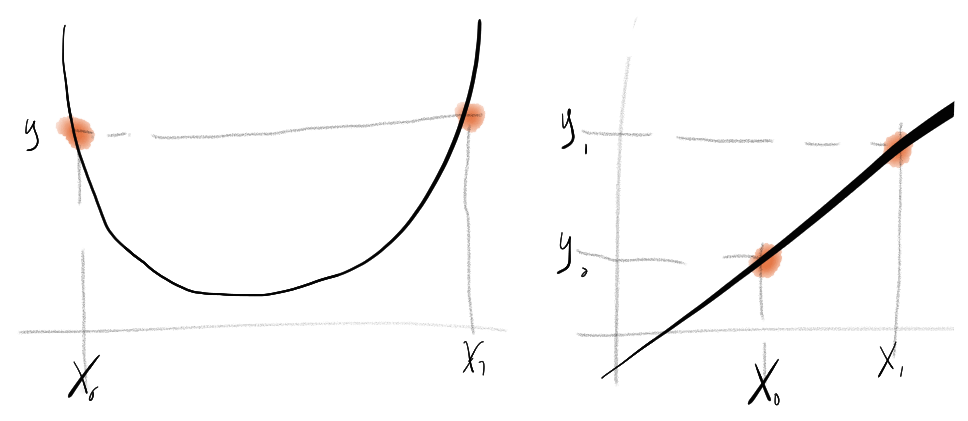
\includegraphics[width=0.9\textwidth]{./imagenes/1.PNG}
            \caption{\label{fig:indis}Grafica de dos salidas de un sistema bajo estados indistinguibles y distinguibles.}
        \end{figure*}

		\begin{teorema}
			Un sistema es completamente observable si y solamente si, la matriz de observabilidad:

			\begin{equation}
				Ob =
				\begin{pmatrix}
					C \\
					CA \\
					\vdots \\
					CA^{n-1}
				\end{pmatrix}
			\end{equation}

			tiene rango igual a la dimensión del espacio de estado.
		\end{teorema}

		\begin{proof}
			Supongamos que el sistema no es completamente observable, entonces existen $x_1$ y $x_2$ estados diferentes ($x_1 \ne x_2$) no distinguibles, es decir:

			\begin{equation*}
				y(x_1, t, u) = y(x_2, t, u) \quad \forall \+ u \quad \forall t \geq 0
			\end{equation*}

			Dado esto, del sistema original podemos sacar la siguiente conclusión:

			\begin{align*}
				\dot{x} &= A x + B u \\
				\dot{x} - A x &= B u \\
				\exp{(-A t)} (\dot{x} - A x) &= \exp{(-A t)} B u \\
				(\exp{(-A t)} x)' &= \exp{(-A t)} B u \\
				\exp{(-A t)} x &= \int_0^t \exp{(-A \tau)} B u(\tau) d\tau + k \\
				x &= \exp{(A t)} \int_0^t \exp{(-A \tau)} B u(\tau) d\tau + k \exp{(A t)}\\
				x &= \int_0^t \exp{A(t - \tau)} B u(\tau) d\tau + \exp{(At)}x_0
			\end{align*}

			teniendo que la ecuación de salida es:

			\begin{align*}
				y(x_1) &= C e^{A t} x_1 + \int_0^t e^{A(t - \tau)} B u(\tau) d\tau \\
				y(x_2) &= C e^{A t} x_2 + \int_0^t e^{A(t - \tau)} B u(\tau) d\tau
			\end{align*}

			pero tenemos que $y(x_1) = y(x_2)$, por lo que:

			\begin{equation*}
				C \exp{(A t)} (x_1 - x_0) = 0 \quad x_1 \ne x_0
			\end{equation*}

			Dada esta ecuación, podemos construir un sistema derivando de la siguiente manera:

			\begin{align*}
				C \exp{(A t)} (x_1 - x_0) &= 0 \\
				C A \exp{(A t)} (x_1 - x_0) &= 0 \\
				&\vdots \\
				C A^{n-1} \exp{(A t)} (x_1 - x_0) &= 0
			\end{align*}

			reemplazando a $x_1 - x_0$ simplemente con $x$, tenemos que:

			\begin{equation*}
				\begin{pmatrix}
					C \\
					CA \\
					\vdots \\
					CA^{n-1}
				\end{pmatrix} \exp{(A t)} x = 0
			\end{equation*}

			y ya que por definición $\exp{(A T)} \ne 0$, tenemos que:

			\begin{equation*}
				\begin{pmatrix}
					C \\
					CA \\
					\vdots \\
					CA^{n-1}
				\end{pmatrix} x = 0
			\end{equation*}

			es decir:

			\begin{equation*}
				x \in \ker
				\begin{pmatrix}
					C \\
					CA \\
					\vdots \\
					CA^{n-1}
				\end{pmatrix}
			\end{equation*}

			y como $x_1 - x_0 = x \ne 0$, sabemos que:

			\begin{equation*}
				\dim{\ker}
				\begin{pmatrix}
					C \\
					CA \\
					\vdots \\
					CA^{n-1}
				\end{pmatrix} \ne 0
			\end{equation*}

			Por otro lado, tenemos que:

			\begin{equation*}
				\dim{Ob} = \dim
				\begin{pmatrix}
					C \\
					CA \\
					\vdots \\
					CA^{n-1}
				\end{pmatrix} = n
			\end{equation*}

			y dado que:

			\begin{align*}
				\dim{Ob} &= \dim{\ker{Ob}} + \dim{\imagen{Ob}} \\
				n &= a + b \\
			\end{align*}

			con $a \ne 0$, lo que nos da que $\rango{Ob} < n$, lo cual no es posible si el sistema es completamente observable, luego la hipotesis es falsa y concluimos que para que el sistema sea completamente observable $Ob$ debe ser de rango pleno.
		\end{proof}

%-------------------------------------------------------------------------------
%	EMPIEZA SECCION
%-------------------------------------------------------------------------------
\newpage
\section{Operadores lineales}

	\subsection{Definiciones}

		\begin{definicion}
			Sea $V$ un espacio vectorial con una transformación lineal $T \colon V \to V$.
			A $T$ se le llama operador lineal.
		\end{definicion}

		\begin{observacion}
			Si $T$ es operador lineal en $V$, escribimos:

			\begin{equation}
				T^2 = T \circ T
			\end{equation}

			y en general:

			\begin{equation}
				T^n = \overbrace{T \circ T \circ T \dots \circ T}^{n \text{ veces}}
			\end{equation}

			o bien:

			\begin{equation}
				T^n = T^{n-1} \circ T
			\end{equation}

			para $n \geq 2$.
		\end{observacion}

		\begin{proposicion}
			Sea $T \colon V \to W$ una transformación lineal, entonces el hecho de que $T$ se isomorfismo, implica que $T$ sea invertible y bisceversa, es decir:

			\begin{equation}
				T \text{ es isomorfismo} \iff T \text{ es invertible}
			\end{equation}

			Recordando que $T$ es invertible si existe una $T^{-1}$ por la izquierda y por la derecha, tal que:

			\begin{align}
				T^{-1} \circ T &= I_V \nonumber \\
				T \circ T^{-1} &= I_W
			\end{align}
		\end{proposicion}

		\begin{proof}
			Para comprobar esta proposición empezaremos asumiendo que $T$ es invertible, esto es existe un $T^{-1}$.

			Supongamos ahora que:

			\begin{equation}
				T(x_1) = T(x_2) \quad x_1, x_2 \in V
			\end{equation}

			si componemos con $T^{-1}$ por la izquierda:

			\begin{align*}
				T^{-1} \circ T(x_1) &= T^{-1} \circ T(x_2) \\
				I_V(x_1) &= I_V(x_2) \\
				x_1 &= x_2
			\end{align*}

			por lo que $T$ es inyectiva.

			Si ahora, tenemos un $y \in W$ tal que $x = T^{-1}(y)$, por lo que:

			\begin{equation*}
				T(x) = T(T^{-1}(y)) = T \circ T^{-1}(y) = I_W(y) = y
			\end{equation*}

			Por lo que $T$ es suprayectiva, y por lo tanto $T$ es isomorfismo.
		\end{proof}

		\begin{proposicion}
			Si $T$ es transformación lineal de $V$ en $W$ y $T$ es invertible, entonces: $T^{-1} \colon W \to V$ es lineal.
		\end{proposicion}

%-------------------------------------------------------------------------------
%	EMPIEZA SECCION
%-------------------------------------------------------------------------------
\newpage
\section{Funcionales lineales}

	\subsection{Definiciones}

		\begin{lema}
			Sea $\mathbb{F}$ un campo y $V$ un espacio vectorial sobre $\mathbb{F}$.

			$\mathbb{F}$ como espacio vectorial sobre $\mathbb{F}$ tiene dimensión uno.
		\end{lema}

		\begin{proof}
			Sea $\{1\}$ un generador y un elemento linealmente independiente.

			\begin{enumerate}
				\item $k \cdot 1 = 0 \implies k = 0$, por lo que $1$ es linealmente independiente.
				\item $a \in \mathbb{F}$, $a = a \cdot 1$, por lo que $1$ es generador.
			\end{enumerate}

			por lo que $1$ es base y $\mathbb{F}$ es de dimensión $1$.
		\end{proof}

		\begin{definicion}
			Un funcional lineal de $V$ es una transformación lineal, tal que:

			\begin{equation}
				f \colon V \to \mathbb{F}
			\end{equation}
		\end{definicion}

%-------------------------------------------------------------------------------
%	EMPIEZA SECCION
%-------------------------------------------------------------------------------
\newpage
\section{Espacio dual}

	\subsection{Definiciones}

		\begin{definicion}
			El espacio dual de $V$ es denotado por $V^*$, tal que:

			\begin{equation}
				V^* = \left\{ f \mid f \text{ es funcional lineal de } V \right\} = \mathcal{L}(V, \mathbb{F})
			\end{equation}
		\end{definicion}

		\begin{observacion}
			Sea $V, W$ espacios vectoriales sobre $\mathbb{F}$, si $\dim{V} = n$ y $\dim{W} = m$.

			\begin{equation}
				\dim{\mathcal{L}(V, W)} = m \cdot n
			\end{equation}
		\end{observacion}

		\begin{observacion}
			Utilizando la observación anterior, podemos decir que:

			\begin{equation} 
				\dim{V^*} = \dim{\mathcal{L}(V, \mathbb{F})} = 1 \cdot n = n = \dim{V}
			\end{equation}

			por lo que $V^*$ es isomorfo a $V$.
		\end{observacion}

		\begin{definicion}
			Si $\{ \alpha_1, \alpha_2, \dots, \alpha_n \}$ es una base de $V$, consideremos $\{1\}$ una base para $\mathbb{F}$, entonces definimos:

			\begin{equation} \label{eq:func1}
				f_i(\alpha_k) = \delta_{ik} =
				\begin{cases}
					1 & \text{ Si } i = k \\
					0 & \text{ Si } i \ne k
				\end{cases}
			\end{equation}
		\end{definicion}

		\begin{definicion}
			Si $\{ \alpha_1, \alpha_2, \dots, \alpha_n \}$ es base de $V$, la base $\{ f_1, f_2, \dots, f_n \}$ de $V^*$ dada por~\ref{eq:func1} se llama base dual a la base $\{ \alpha_1, \alpha_2, \dots, \alpha_n \}$
		\end{definicion}

		\begin{ejemplo}
			\faltante{Falta escribir ejemplo}
		\end{ejemplo}

		\begin{ejemplo}
			\faltante{Falta escribir ejemplo}
		\end{ejemplo}

		\begin{ejemplo}
			\faltante{Falta escribir ejemplo}
		\end{ejemplo}

		\begin{ejemplo}
			\faltante{Falta escribir ejemplo}
		\end{ejemplo}

		\begin{proposicion}
			Si $\{f_i\}_{1 \leq i \leq n}$ es la base dual de $V^*$ a la base $\{\alpha_i\}_{1 \leq i \leq n}$ de $V$, entonces tenemos que:

			\begin{enumerate}
				\item Si $f \in V^*$, entonces $f = \sum_{i=1}^n f(\alpha_i) f_i$
				\item Si $\alpha \in V$, entonces $\alpha = \sum_{i=1}^n f_i(\alpha) \alpha_i$
			\end{enumerate}
		\end{proposicion}

		\begin{proof}
			Sea $\alpha \in V$ de la forma:

			\begin{equation*}
				\alpha = a_1 \alpha_1 + a_2 \alpha_2 + \dots + a_n \alpha_n
			\end{equation*}

			\begin{align*}
				\left[ \sum_{i=1}^n f(\alpha_i) f_i \right] (\alpha) &= \sum_{i=1}^n f(\alpha_i) f_i(\alpha) \\
				&= \sum_{i=1}^n f(\alpha_i) f_i(a_1 \alpha_1 + a_2 \alpha_2 + \dots + a_n \alpha_n) \\
				&= \sum_{i=1}^n f_i(\alpha) a_i
			\end{align*}
		\end{proof}

		\begin{ejercicio}
			Determinar explicitamente la base dual a la base $v_1 = \begin{pmatrix} 1 & 1 & 1 \end{pmatrix}$, $v_2 = \begin{pmatrix} 0 & 1 & 1 \end{pmatrix}$ y $v_3 = \begin{pmatrix} 0 & 0 & 1 \end{pmatrix}$ de $\mathbb{R}^3$.
		\end{ejercicio}

		\begin{ejercicio}
			Sea $f$ el funcional lineal en $\left( \mathbb{R}^3 \right)^*$ dado por:

			\begin{equation*}
				f(\begin{pmatrix} x & y & z \end{pmatrix}) = x + y + z
			\end{equation*}

			Exprese $f$ como combinación lineal de la base dual encontrada en $a$.
		\end{ejercicio}

%-------------------------------------------------------------------------------
%	EMPIEZA SECCION
%-------------------------------------------------------------------------------

\section{Teorema de Cayley - Hamilton}

	\begin{definicion}
		Toda matriz es un cero de su polinomio caracteristico
	\end{definicion}

	\begin{proof}
		Sea $A$ una matriz cuadrada arbitraria de tamaño $n \times n$ y $P(\lambda)$ su polinomio caracteristico, es decir:

		\begin{equation*}
			P(\lambda) = |\lambda I - A| = \lambda^n + \dots + a_1 \lambda + a_0
		\end{equation*}

		Supongamos ahora que $B(\lambda)$ representa a la adjunta de la matriz $\lambda I - A$, entonces los elementos de $B(\lambda)$ son los cofactores de la matriz $\lambda I - A$ y por lo tanto son polinomios en $\lambda$ de grado no mayor que $n-1$.
		Por lo tanto $B(\lambda)$ tiene la forma:

		\begin{equation*}
			B(\lambda) = B_{n-1} \lambda^{n-1} + \dots + B_1 \lambda + B_0
		\end{equation*}

		donde $B_i$ son matrices $n \times n$ sobre un campo $K$.

		Por la propiedad fundamental de la adjunta:

		\begin{equation*}
			(\lambda I - A) B(\lambda) = |\lambda I - A| I
		\end{equation*}

		de aqui tenemos que:

		\begin{equation*}
			(\lambda I - A) (B_{n-1} \lambda^{n-1} + \dots + B_1 \lambda + B_0) = (\lambda^n + \dots + a_1 \lambda + a_0) I
		\end{equation*}

		Quitando los parentesis e igualando los coeficientes de las mismas potencias de $\lambda$, tenemos:

		\begin{align*}
			B_{n-1} &= I \tag{$\lambda^n$} \\
			B_{n-2} - A B_{n-1} &= a_{n-1} I \tag{$\lambda^{n-1}$} \\
			B_{n-3} - A B_{n-2} &= a_{n-2} I \tag{$\lambda^{n-2}$} \\
			&\vdots \\
			B_0 - A B_1 &= a_1 I \tag{$\lambda^1$} \\
			- A B_0 &= a_0 I \tag{$\lambda^0$}
		\end{align*}

		Si ahora multiplicamos estas ecuaciones matriciales por $A^n, A^{n-1}, \dots, A, I$, tendremos:

		\begin{align*}
			A^n B_{n-1} &= A^n \tag{$\lambda^n$} \\
			A^{n-1} B_{n-2} - A^n B_{n-1} &= a_{n-1} A^{n-1} \tag{$\lambda^{n-1}$} \\
			A^{n-2} B_{n-3} - A^{n-1} B_{n-2} &= a_{n-2} A^{n-2} \tag{$\lambda^{n-2}$} \\
			&\vdots \\
			A B_0 - A^2 B_1 &= a_1 I \tag{$\lambda^1$} \\
			- A B_0 &= a_0 I \tag{$\lambda^0$}
		\end{align*}

		Y al sumar todas las ecuaciones tendremos:

		\begin{equation*}
			0 = A^n + a_{n-1} A^{n-1} + a_{n-2} A^{n-2} + \dots + a_1 A + a_0 I = P(A)
		\end{equation*}
	\end{proof}

	\begin{ejemplo}
		El polinomio caracteristico de la matriz:

		\begin{equation*}
			A =
			\begin{pmatrix}
				1 & 2 \\
				3 & 2
			\end{pmatrix}
		\end{equation*}

		Obtenemos su polinomio caracteristico:

		\begin{align*}
			|\lambda I - A| &= \det{(\lambda I - A)} = |A - \lambda I| \\
			&=
			\begin{vmatrix}
				1 - \lambda & 2 \\
				3 & 2 - \lambda
			\end{vmatrix} = (1 - \lambda)(2 - \lambda) - 6 \\
			&= \lambda^2 - 3 \lambda - 4 = P(\lambda)
		\end{align*}

		y podemos ver que $A$ es un cero de $P(\lambda)$.

		\begin{align*}
			P(A) &= A^2 - 3 A - 4I =
			\begin{pmatrix}
				1 & 2 \\
				3 & 2
			\end{pmatrix}^2 - 3
			\begin{pmatrix}
				1 & 2 \\
				3 & 2
			\end{pmatrix} - 4
			\begin{pmatrix}
				1 & 0 \\
				0 & 1
			\end{pmatrix} \\
			&=
			\begin{pmatrix}
				7 & 6 \\
				9 & 10
			\end{pmatrix} -
			\begin{pmatrix}
				3 & 6 \\
				9 & 6
			\end{pmatrix} -
			\begin{pmatrix}
				4 & 0 \\
				0 & 4
			\end{pmatrix} \\
			&=
			\begin{pmatrix}
				0 & 0 \\
				0 & 0
			\end{pmatrix}
		\end{align*}
	\end{ejemplo}

%-------------------------------------------------------------------------------
%	EMPIEZA SECCION
%-------------------------------------------------------------------------------
\newpage
\section{Diagonalización}

	\subsection{Definiciones}

		\begin{definicion}
			Sea $V$ un espacio vectorial de dimensión finita $n$ y $T \colon V \to V$ un operador lineal, entonces $T$ puede representarse por una matriz $n \times n$ $A$.
			Por esta razón en algunas ocasiones nos vamos a referir a valores y vectores propios de matrices $n \times n$.
		\end{definicion}

		\begin{teorema}
			Sea $A$ una matriz $n \times n$. Entonces $\lambda$ es un valor propio de $A$ si y solo si:

			\begin{equation}
				p(\lambda) = \det{(A - \lambda I)} = 0
			\end{equation}
		\end{teorema}

		\begin{proposicion}
			Sabemos que $p(\lambda)$ se puede escribir como:

			\begin{equation}
				p(\lambda) = \lambda^n + a_{n-1} \lambda^{n-1} + \dots + a_1 \lambda + a_0 = 0
			\end{equation}

			Esta ecuación tiene $n$ raices, varias de las cuales pueden repetirse.

			Si $\lambda_1, \lambda_2, \dots, \lambda_k$ son las diferentes raices de $p(\lambda)$ con multiplicidad $r_1, r_2, \dots, r_k$ respectivamente, entonces $p(\lambda)$ puede factorizarse como:

			\begin{equation}
				p(\lambda) = (\lambda - \lambda_1)^{r_1} (\lambda - \lambda_2)^{r_2} \dots (\lambda - \lambda_k)^{r_k} = 0
			\end{equation}

			en donde los numeros $r_1, r_2, \dots, r_k$ se llaman multiplicidades algebraicas de los valores propios $\lambda_1, \lambda_2, \dots, \lambda_k$ respectivamente.

			Sea $\lambda$ un valor propio de $T$ y sea:

			\begin{equation}
				E_{\lambda} = \left\{ v \colon Tv = \lambda v \right\} = \left\{ v \colon (T - \lambda I) v = 0 \right\}
			\end{equation}

			El subespacio $E_{\lambda}$ (pues es el nucleo de la transformación lineal $T - \lambda I$) se llama espacio propio de $T$ correspondiente al valor propio $\lambda$.

			Como $E_\lambda$ es un subespacio entonces $0 \in E_{\lambda}$, pero $\dim{E_{\lambda}} > 0$ pues por definición, si $\lambda$ es un valor propio, entonces existe un vector propio diferente de cero correspondiente a $\lambda$.
		\end{proposicion}

		\begin{teorema}
			Sea $V$ un espacio vectorial de dimensión finita $n$ y $T \colon V \to V$ un operador lineal y sean $\lambda_1, \lambda_2, \dots, \lambda_n$ valores propios diferentes de $T$ con sus correspondientes vectores propios $v_1, v_2, \dots, v_n$.
			Entonces $v_1, v_2, \dots, v_n$ son linealmente independientes.
		\end{teorema}

		\begin{proposicion}
			Sea $A$ una representación matricial de $T$. Supongamos que $A$ es una matriz de $3 \times 3$.

			\begin{enumerate}
				\item Si $A$ tiene tres diferentes valores propios $\lambda_1, \lambda_2, \lambda_3$ (cada uno con multiplicidad algebraica uno), entonces, por el primer teorema, sus respectivos vectores propios $v_1, v_2, v_3$ son linealmente independientes.
				\item Si $A$ tiene dos vectores propios $\lambda_1$ y $\lambda_2$ con multiplicidad algebraica uno y dos respectivamente.
				Entonces $\dim{E_{\lambda_2}} \leq 2$, porque de otra manera, podriamos tener al menos cuatro vectores linealmente independientes en un espacio de tres dimensiones.
				Es decir, para $\lambda_2$ puede haber uno o dos vectores propios linealmente independientes.
				\item Si $A$ tiene un valor propio $\lambda$ con multiplicidad algebraica tres, entonces $\dim{E_{\lambda}} \leq 3$, es decir, puede haber uno, dos o tres vectores propios linealmente independientes.
			\end{enumerate}
		\end{proposicion}

		\begin{teorema}
			Sea $\lambda$ un valor propio para $T$ operador lineal en un espacio vectorial de dimensión finita, entonces:

			\begin{equation}
				1 \leq \dim{E_{\lambda}} \leq \text{multiplicidad algebraica de } \lambda
			\end{equation}
		\end{teorema}

		\begin{ejemplo}
			Sea $A$:

			\begin{equation*}
				A =
				\begin{pmatrix}
					-3 & 3 & -2 \\
					-7 & 6 & -3 \\
					1 & -1 & 2
				\end{pmatrix}
			\end{equation*}

			por lo que el determinante de $A - \lambda I$ es:

			\begin{equation*}
				\det{(A - \lambda I)} = (\lambda - 2)^2 (\lambda - 1)
			\end{equation*}

			y los valores propios de $A$ son $\lambda_1 = 2$ con multiplicidad algebraica dos y $\lambda_2 = 1$ con multiplicidad algebraica uno.

			Tenemos pues, el subespacio $E_{\lambda_1}$:

			\begin{align*}
				E_{\lambda_1} &= \ker{(A - \lambda_1 I)} = \ker{(A - 2I)} \\
				&= \left\{ \begin{pmatrix} x_1 \\ x_2 \\ x_3 \end{pmatrix} \colon \begin{pmatrix} -5 & 3 & -2 \\ -7 & 4 & -3 \\ 1 & -1 & 0 \end{pmatrix} \begin{pmatrix} x_1 \\ x_2 \\ x_3 \end{pmatrix} = \begin{pmatrix} 0 \\ 0 \\ 0 \end{pmatrix} \right\}
			\end{align*}

			Resolviendo este sistema, se obtiene el único vector propio linealmente independiente $v_1 = \begin{pmatrix} 1 \\ 1 \\ -1 \end{pmatrix}$, por lo que:

			\begin{equation*}
				E_{\lambda_1} = \mathcal{L} \left\{ \begin{pmatrix} 1 \\ 1 \\ -1 \end{pmatrix} \right\}
			\end{equation*}

			y por lo tanto $\dim{E_{\lambda_1}} = 1$

			Ahora, para $E_{\lambda_2}$ tenemos:

			\begin{align*}
				E_{\lambda_2} &= \ker{(A - \lambda_2 I)} = \ker{(A - I)} \\
				&= \left\{ \begin{pmatrix} x_1 \\ x_2 \\ x_3 \end{pmatrix} \colon \begin{pmatrix} -4 & 3 & -2 \\ -7 & 5 & -3 \\ 1 & -1 & 1 \end{pmatrix} \begin{pmatrix} x_1 \\ x_2 \\ x_3 \end{pmatrix} = \begin{pmatrix} 0 \\ 0 \\ 0 \end{pmatrix} \right\}
			\end{align*}

			y tenemos que el vector propio linealmente independiente asociado a $\lambda_2$ es $v_2 = \begin{pmatrix} 1 \\ 2 \\ 1 \end{pmatrix}$, por lo que:

			\begin{equation*}
				E_{\lambda_2} = \mathcal{L} \left\{ \begin{pmatrix} 1 \\ 2 \\ 1 \end{pmatrix} \right\}
			\end{equation*}

			y por lo tanto $\dim{E_{\lambda_2}} = 1$.
		\end{ejemplo}

		\begin{definicion}
			Dos matrices $A$ y $B$ de $n \times n$ se llaman equivalentes si existe una matriz invertible $Q$ de $n \times n$ tal que:

			\begin{equation}
				B = Q^{-1} A Q
			\end{equation}

			en donde $Q$ se llama matriz de transformación.
		\end{definicion}

		\begin{teorema}
			Si $A$ y $B$ son matrices equivalentes de $n \times n$, $A$ y $B$ tienen el mismo polinomio caracteristico y por consiguiente tienen los mismos valores propios.
		\end{teorema}

		\begin{definicion}
			Una matriz $A$ de $n times n$ es diagonalizable si existe una matriz diagonal $D$ tal que $A$ es equivalente a $D$, es decir:

			\begin{equation}
				D = Q^{-1} A Q
			\end{equation}

			donde $Q$ es una matriz invertible.
		\end{definicion}

		\begin{observacion}
			Si $D$ es una matriz diagonal, entonces sus valores propios son las componentes de su diagonal.
		\end{observacion}

		\begin{observacion}
			Si $A$ es equivalente a $D$ tenemos los mismos valores propios, debido al teorema 2.8.4.
		\end{observacion}

		\begin{observacion}
			Englobando estos dos ultimos resultados, observamos que si $A$ es diagonalizable, entonces $A$ es equivalente a una matriz diagonal y las componentes de la diagonal son los valores propios de $A$.
		\end{observacion}

		\begin{teorema}
			Una matriz $A$ de $n \times n$ es diagonalizable si y solo si tiene $n$ vectores propios linealmente independientes.

			En este caso, la matriz diagonal $D$ equivalente a la matriz $A$ esta dada por:

			\begin{equation}
				D =
				\begin{pmatrix}
					\lambda_1 & 0 & 0 & \dots 0 \\
					0 & \lambda_2 & 0 & \dots 0 \\
					0 & 0 & \lambda_3 & \dots 0 \\
					\vdots & \vdots & \vdots & & \vdots \\
					0 & 0 & 0 & \dots & \lambda_n
				\end{pmatrix}
			\end{equation}

			donde $\lambda_1, \lambda_2, \dots, \lambda_n$ son los valores propios de $A$.
			Además, si $Q$ es una matriz cuyas columnas son vectores propios linealmente independientes de $A$, entonces:

			\begin{equation}
				D = Q^{-1} A Q
			\end{equation}
		\end{teorema}

		\begin{corolario}
			Si la matriz $A$ de $n \times n$ tiene $n$ valores propios diferentes, entonces $A$ esdiagonalizable.
		\end{corolario}

		\begin{ejemplo}
			Sea $A$:

			\begin{equation*}
				A =
				\begin{pmatrix}
					1 & -1 & 4 \\
					3 & 2 & -1 \\
					2 & 1 & -1
				\end{pmatrix}
			\end{equation*}

			por lo que tenemos que:

			\begin{equation*}
				\det{(A - \lambda I)} = - (\lambda - 1)(\lambda + 2)(\lambda - 3)
			\end{equation*}

			por lo que sus valores propios son $\lambda_1 = 1$, $\lambda_2 = -2$ y $\lambda_3 = 3$.

			Como son tres valores propios diferentes, entonces por el teorema 2.8.2, tenemos que hay tres vectores propios linealmente independientes, que pueden ser:

			\begin{align*}
				v_1 &= \begin{pmatrix} -1 \\ 4 \\ 1 \end{pmatrix} \\
				v_1 &= \begin{pmatrix} 1 \\ -1 \\ -1 \end{pmatrix} \\
				v_1 &= \begin{pmatrix} 1 \\ 2 \\ 1 \end{pmatrix}
			\end{align*}

			entonces, por el teorema 2.8.5, $A$ es diagonalizable y la matriz de transformación $Q$ es:

			\begin{equation*}
				Q =
				\begin{pmatrix}
					-1 & 1 & 1 \\
					4 & -1 & 2 \\
					1 & -1 & 1
				\end{pmatrix}
			\end{equation*}

			y podemos ver que:

			\begin{align*}
				Q^{-1} A Q &= -\frac{1}{6}
				\begin{pmatrix}
					1 & -2 & 3 \\
					-2 & -2 & 6 \\
					-3 & 0 & -3
				\end{pmatrix}
				\begin{pmatrix}
					1 & -1 & 4 \\
					3 & 2 & -1 \\
					2 & 1 & -1
				\end{pmatrix}
				\begin{pmatrix}
					-1 & 1 & 1 \\
					4 & -1 & 2 \\
					1 & -1 & 1
				\end{pmatrix} \\
				&=
				\begin{pmatrix}
					1 & 0 & 0 \\
					0 & -2 & 0 \\
					0 & 0 & 3
				\end{pmatrix} = D
			\end{align*}
		\end{ejemplo}

		\begin{ejemplo}
			Sea $A$:

			\begin{equation*}
				A =
				\begin{pmatrix}
					3 & 2 & 4 \\
					2 & 0 & 2 \\
					4 & 2 & 3
				\end{pmatrix}
			\end{equation*}

			por lo que tenemos que:

			\begin{equation*}
				\det{(A - \lambda I)} = -(\lambda + 1)^2(\lambda - 8) = 0
			\end{equation*}

			Entonces los valores propios son $\lambda_1 = -1$ con multiplicidad algebraica dos y $\lambda_2 = 8$ con multiplicidad algebraica uno.

			Para $\lambda_2$ se obtiene un vector propio linealmente independiente:

			\begin{equation*}
				v_1 =
				\begin{pmatrix}
					2 \\
					1 \\
					2
				\end{pmatrix}
			\end{equation*}

			y para $\lambda_1$ se tienen dos vectores propios linealmente independientes:

			\begin{align*}
				v_2 &= \begin{pmatrix} 1 & -2 & 0 \end{pmatrix} \\
				v_3 &= \begin{pmatrix} 0 & -2 & 1 \end{pmatrix}
			\end{align*}

			por lo que, por el teorema 2.8.5, tenemos que $A$ es diagonalizable, y la matriz $Q$ es:

			\begin{equation*}
				Q =
				\begin{pmatrix}
					2 & 1 & 0 \\
					1 & -2 & -2 \\
					2 & 0 & 1
				\end{pmatrix}
			\end{equation*}

			y tenemos que:

			\begin{align*}
				Q^{-1} A Q &= -\frac{1}{9}
				\begin{pmatrix}
					-2 & -1 & -2 \\
					-5 & 2 & 4 \\
					4 & 2 & -5
				\end{pmatrix}
				\begin{pmatrix}
					3 & 2 & 4 \\
					2 & 0 & 2 \\
					4 & 2 & 3
				\end{pmatrix}
				\begin{pmatrix}
					2 & 1 & 0 \\
					1 & -2 & -2 \\
					2 & 0 & 1
				\end{pmatrix} \\
				&=
				\begin{pmatrix}
					8 & 0 & 0 \\
					0 & -1 & 0 \\
					0 & 0 & -1
				\end{pmatrix} = D
			\end{align*}

			Este ejemplo ilustra que $A$ es diagonalizable aun cuando sus valores propios no son diferentes.
		\end{ejemplo}

		\begin{ejemplo}
			En el ejemplo 2.8.1, la matriz $A$ de $3 \times 3$ tiene solo dos vectores propios linealmente independientes, entonces no es posible hallar la matriz de transformación $Q$, por tanto, por el teorema 2.8.5, la matriz $A$ no es diagonalizable.

			Las matrices de $n \times n$ con $n$ vectores propios linealmente independientes pueden ser llevados a una matriz diagonal mediante una transformación de equivalencia.

			Como la mayoria de los polinmios  tienen diferentes raices, la mayoria de las matrices tendrán diferentes valores propios y por tanto son diagonalizables.

			Las matrices que no son diagonalizables (esto es, que no tienen $n$ vectores propios linealmente independientes) aparecen en ciertas aplicaciones. En este caso todavia es posible mostrar que la matriz es equivalente a otra matriz mas simple, pero la nueva matriz ya no es diagonal y la matriz de transformación $Q$ es mas dificil de obtener.
		\end{ejemplo}

%-------------------------------------------------------------------------------
%	EMPIEZA SECCION
%-------------------------------------------------------------------------------
\newpage
\section{Forma canónica de Jordan}
	\subsection{Definiciones}

		\begin{definicion}
			Aun cuando no todo operador $T$ es lineal es diagonalizable, es posible hallar una base $\beta$ para el espacio vectorial $V$ de dimensión $n$ tal que la representación matricial de $A$ de $n \times n$ de $T$ es equivalente a:

			\begin{equation}
				J =
				\begin{pmatrix}
					J_1 & 0 & \dots 0 \\
					0 & J_2 & \dots 0 \\
					\vdots & \vdots & & \vdots \\
					0 & 0 & \dots & J_n
				\end{pmatrix}
			\end{equation}

			donde $J_i$ es una matriz diagonal de la forma $(\lambda_i)$, o bien de la forma:

			\begin{equation*}
				J_i =
				\begin{pmatrix}
					\lambda_i & 1 & 0 & \dots & 0 & 0 \\
					0 & \lambda_i & 1 & \dots & 0 & 0 \\
					0 & 0 & \lambda_i & \dots & 0 & 0 \\
					\vdots & \vdots & \vdots & & \vdots & \vdots \\
					0 & 0 & 0 & \dots & \lambda_i & 1 \\
					0 & 0 & 0 & \dots & 0 & \lambda_i \\
				\end{pmatrix}
			\end{equation*}

			para algun valor propio $\lambda_i$ de $A$.

			A $J_i$ le llamamos bloque de Jordan correspondiente a $\lambda_i$.
			$\beta_i$ es la base correspondiente al bloque $J_i$.
			$J$ se le llama forma canónica de Jordan de $A$.
			$\beta$ se llama base canónica de Jordan.
		\end{definicion}

		\begin{observacion}
			Cada bloque de Jordan $J_i$ es casi una matriz diagonal, de hecho $J$ es una matriz diagonal si y solo si, cada $J_i$ es de la forma $(\lambda_i)$.
		\end{observacion}

		\begin{ejemplo}
			Sea $A$:

			\begin{equation*}
				A =
				\begin{pmatrix}
					4 & \vdots & 0 & 0 & 0 & \vdots & 0 \\
					\dots & & \dots & \dots & \dots & & \dots \\
					0 & \vdots & -3 & 1 & 0 & \vdots & 0 \\
					0 & \vdots & 0 & -3 & 1 & \vdots & 0 \\
					0 & \vdots & 0 & 0 & -3 & \vdots & 0 \\
					\dots & & \dots & \dots & \dots & & \dots \\
					0 & \vdots & 0 & 0 & 0 & \vdots & 7 
				\end{pmatrix}
			\end{equation*}

			Los bloques de Jordan están marcados por las lineas punteadas.
			La multiplicidad algebraica de cada valor propio $\lambda_i$ es el numero de veces que el valor propio aparece en la diagonal de $J_i$.
		\end{ejemplo}

		\begin{proposicion}
			Sea $\lambda_i$ un valor propio de $A$ tal que $\dim{E_{\lambda_i}} = s_i$, entonces el numero de unos arriba de la diagonal de la forma canónica de Jordan es:

			\begin{equation}
				n - \sum_{i=1}^k s_i
			\end{equation}

			donde $k$ es el numero de valores propios.
		\end{proposicion}

		\begin{ejemplo}
			Si el polinomio caracteristico de $A$ es $(\lambda - 2)^3(\lambda + 3)$, entonces $\lambda_1 = 2$ con multiplicidad algebraica tres, entonces $E_{\lambda_1} \leq 3$, y $\lambda_2 = -3$ con multiplicidad algebraica uno, entonces $\dim{E_{\lambda_2}} = 1$.

			Como $\dim{E_{\lambda_1}} \leq 3$, entonces pueden haber uno, dos o tres vectores propios linealmene independientes para $\lambda_1$.
			Para $\lambda_2$ siempre hay un vector propio independiente.

			Por tanto las posibles formas canónicas de Jordan de $A$ son:

			\begin{enumerate}
				\item Supongamos que $\dim{E_{\lambda_1}} = 1$, entonces:
				\begin{equation*}
					J =
					\begin{pmatrix}
						2 & 1 & 0 & 0 \\
						0 & 2 & 1 & 0 \\
						0 & 0 & 2 & 0 \\
						0 & 0 & 0 & -3
					\end{pmatrix}
				\end{equation*}
				\item Supongamos que $\dim{E_{\lambda_1}} = 2$, entonces:
				\begin{equation*}
					J =
					\begin{pmatrix}
						2 & 1 & 0 & 0 \\
						0 & 2 & 0 & 0 \\
						0 & 0 & 2 & 0 \\
						0 & 0 & 0 & -3
					\end{pmatrix}
				\end{equation*}
				\item Supongamos que $\dim{E_{\lambda_1}} = 3$, entonces:
				\begin{equation*}
					J =
					\begin{pmatrix}
						2 & 0 & 0 & 0 \\
						0 & 2 & 0 & 0 \\
						0 & 0 & 2 & 0 \\
						0 & 0 & 0 & -3
					\end{pmatrix}
				\end{equation*}
			\end{enumerate}

			En las columnas donde aparecen los unos arriba del valor propio indica que hay vectores que no son propios.
			Por ejemplo en el inciso 1, las columnas $2$ y $3$ indican que para $\lambda_1$ hay dos vectores que no son propios, mientras que en el inciso 3, todos los vectores son propios.
		\end{ejemplo}

		\begin{teorema}
			Sea $A$ una matriz de $n \times n$, entonces existe una matriz invertible $Q$ de $n \times n$ tal que:

			\begin{equation}
				Q^{-1} A Q = J
			\end{equation}

			donde $J$ es una matriz de Jordan cuyos elementos diagonales son valores propios de $A$.

			$J$ es unica excepto por el orden en que aparecen los bloques de Jordan.
		\end{teorema}

		\begin{ejemplo}
			Del ejemplo 2.9.2, si $A$ es equivalente a $J$, entonces $A$ tambien es equivalente a:

			\begin{equation*}
				J =
				\begin{pmatrix}
					-3 & 0 & 0 & 0 \\
					0 & 2 & 1 & 0 \\
					0 & 0 & 2 & 1 \\
					0 & 0 & 0 & 2
				\end{pmatrix}
			\end{equation*}

			Esto es, los bloques de Jordan son los mismos, pero se puede cambiar el orden en que se escriben.
		\end{ejemplo}

		\begin{ejemplo}
			Sea $p_2(\mathbb{R})$ el conjunto de los polinomios de segundo grado y sea $\beta$ una base para $p_2(\mathbb{R})$ definida como:

			\begin{equation*}
				\beta = \left\{ x_1, x_2, x_3 \right\} = \left\{ 1, x, x^2 \right\}
			\end{equation*}

			Definamos $T$ como:

			\begin{align*}
				T \colon p_2(\mathbb{R}) &\to p_2(\mathbb{R}) \\
				f &\to f'
			\end{align*}

			Calculamos la representación matricial $A$ de $T$ mediante:

			\begin{align*}
				T(1) &= 0 = 0 \cdot 1 + 0 \cdot x + 0 \cdot x^2 \\
				T(x) &= 1 = 1 \cdot 1 + 0 \cdot x + 0 \cdot x^2 \\
				T(x^2) &= 2x = 0 \cdot 1 + 2 \cdot x + 0 \cdot x^2
			\end{align*}

			Entonces $A$ se define como:

			\begin{equation*}
				A =
				\begin{pmatrix}
					0 & 1 & 0 \\
					0 & 0 & 2 \\
					0 & 0 & 0
				\end{pmatrix}
			\end{equation*}
		\end{ejemplo}

%-------------------------------------------------------------------------------
%	EMPIEZA SECCION
%-------------------------------------------------------------------------------
\newpage
\section{Vectores propios generalizados}

	\subsection{Definiciones}

		\begin{definicion}
			Sea $T$ un operador lineal en un espacio vectorial $V$ de dimensión de dimensión $n$. Un elemento no nulo $v \in V$ se llama vector propio generalizado de $T$ si existe un escalar $\lambda$ tal que:

			\begin{equation}
				(T - \lambda I)^p(v) = 0
			\end{equation}

			para algun $p \in \mathbb{Z}^+$.

			Se dice que $v$ es un vector propio generalizado correspondiente a $\lambda$.
		\end{definicion}

		\begin{ejemplo}
			\faltante{Falta escribir ejemplo}
		\end{ejemplo}

		\begin{definicion}
			Sea $T$ un operador lineal en un espacio vectorial $V$.
			Un subespacio $W$ de $V$ se llama subespacio $T$ - ciclico, si existe un elemento $v \in W$ tal que $W$ es igual al subespacio generado por $\{v, T(v), T^2(v), \dots\}$.

			En este caso decimos que $W$ es generado por $v$.
		\end{definicion}

		\begin{ejemplo}
			\faltante{Falta escribir ejemplo}
		\end{ejemplo}

		\begin{definicion}
			Sea $T$ y $V$ como en la definicion anterior y sea $v$ un vector propio generalizado de $T$ correspondiente al valor propio $\lambda$.
			Si $p$ es el entero positivo mas pequeño tal que:

			\begin{equation}
				(T - \lambda I)^p(v) = 0
			\end{equation}

			entonces el conjunto:

			\begin{equation}
				\left\{ (T - \lambda I)^{p-1}, (T - \lambda I)^{p-2}, \dots, (T - \lambda I)(v), v \right\}
			\end{equation}

			se llama un ciclo de vectores propios generalizados de $T$ que corresponden a $\lambda$.

			Los elementos $(T - \lambda I)^{p-1}$ y $v$ se llaman vector inicial y vector terminal del ciclo respectivamente.

			Se dice que la longitud del ciclo es $p$.
		\end{definicion}
		